\begin{LQ}{Modèle des Concepts}

\LQDescription{
    Le modèle des concepts reprend exactement le modèle de l'environnement, en
    ne se focalisant non plus sur les messages circulant entre les acteurs et
    le système (qui ne sont plus représentés), mais en identifiant les concepts
    du système. Celui ci n'est plus une boîte noire. Il est représenté par une
    sorte de diagramme de classe, chaque classe représentant un concept.
}

\LQSchema{

Le MdC possède fait le lien entre les interaction du système avec les acteurs deu MdE. La différence reside que les message ne sont plus affichés et que le système est representer par un diagramme de classe UML. Les acteurs sont les même que ceux du MdE et sont donc représenter de la meme manière par des “bonhomme” ayant leur cardinalité  au niveau de leur tete. Le systeme est donc un diagramme de classe auquel on lie les acteurs comme si il était une classe (dans un diagramme de classe UML). Dans la classe systeme on definit les attribut qui décrive l’état du système . A l’intérieur de la classe représentant le système sont placées les classes modélisant les concepts. Elles possèdent elles aussi des attributs, mais pas d’opération,
et peuvent éventuellement contenir d’autres concepts (à éviter le plus possible). Chaque acteur est lié à un concept.


}

\begin{figure}
   \centering
   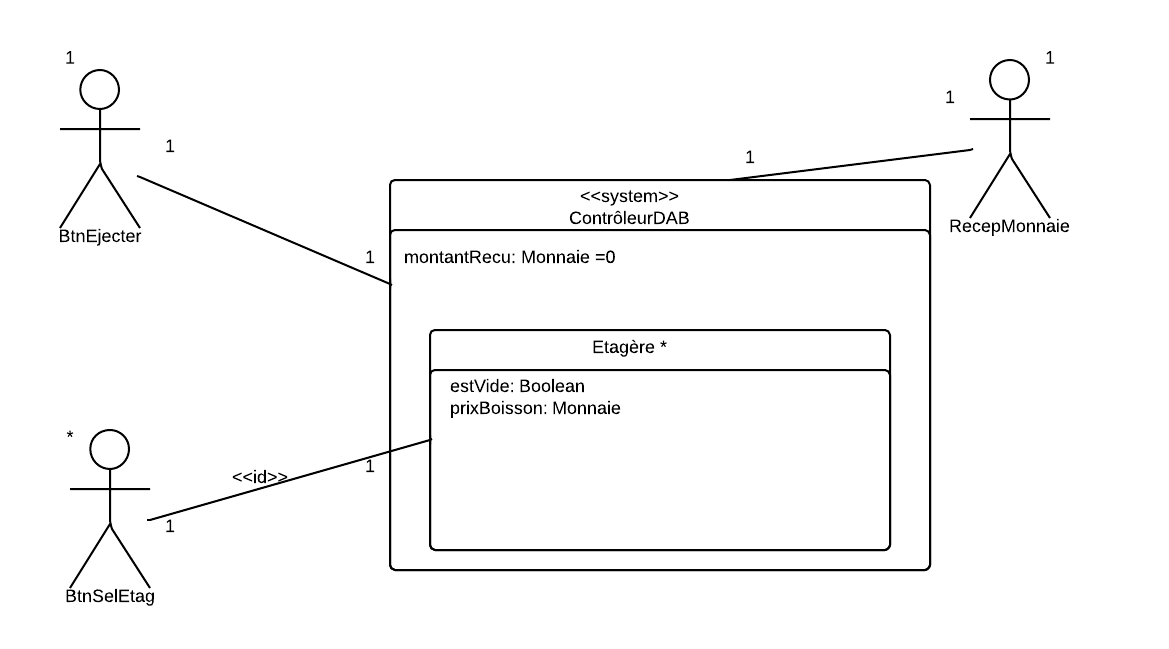
\includegraphics[width=\textwidth]{../images/MdC.png}
   \caption{Schéma du modèle des concept}
\end{figure}


\LQModel{
    Un MdC découle un MdE donc on a autant de MdC que de MdE. Ils utilisent les
    même acteurs et donc la convention de nommage utilisée pour le MdE doit
    être la même pour le MdC
}

\LQBetweenModels{
    Si un acteur se retrouve dans plusieurs MdC, il doit conserver la même
    cardinalité.
}

\end{LQ}
